\documentclass[10pt,a4paper]{article}
\usepackage[T1]{fontenc}
\usepackage[margin=1.9cm]{geometry}
\usepackage{underscore}
\usepackage{amsmath,amssymb}
\usepackage{booktabs,array,graphicx}
\usepackage{tikz}
\usetikzlibrary{arrows.meta,positioning,calc}
\setlength{\parindent}{0pt}
\setlength{\parskip}{5pt}

\tikzset{
  >={Stealth[length=3mm,width=2.4mm]},
  box/.style={draw,rounded corners=2pt,align=center,fill=blue!6,font=\small,inner sep=4pt,minimum width=5.6cm,minimum height=1.1cm},
  hw/.style={draw,dashed,rounded corners=2pt,align=center,fill=green!10,font=\small,inner sep=4pt,minimum width=4.6cm,minimum height=1.1cm},
  data/.style={->,line width=0.9pt},
  lab/.style={font=\scriptsize,fill=white,inner sep=1pt,align=center}
}

\begin{document}

{\LARGE\bfseries Tiny FPGA LM: the accelerator in terms of the neural-network math}

\medskip
This document is the sister of \texttt{fsm_and_lanes.pdf} and \texttt{hardware_schematic.pdf}. It describes the same machine, but every step is stated as arithmetic on the model's vectors and matrices, and each step is then tied to the hardware block that performs it.

\section*{1. The model, end to end}

\begin{center}
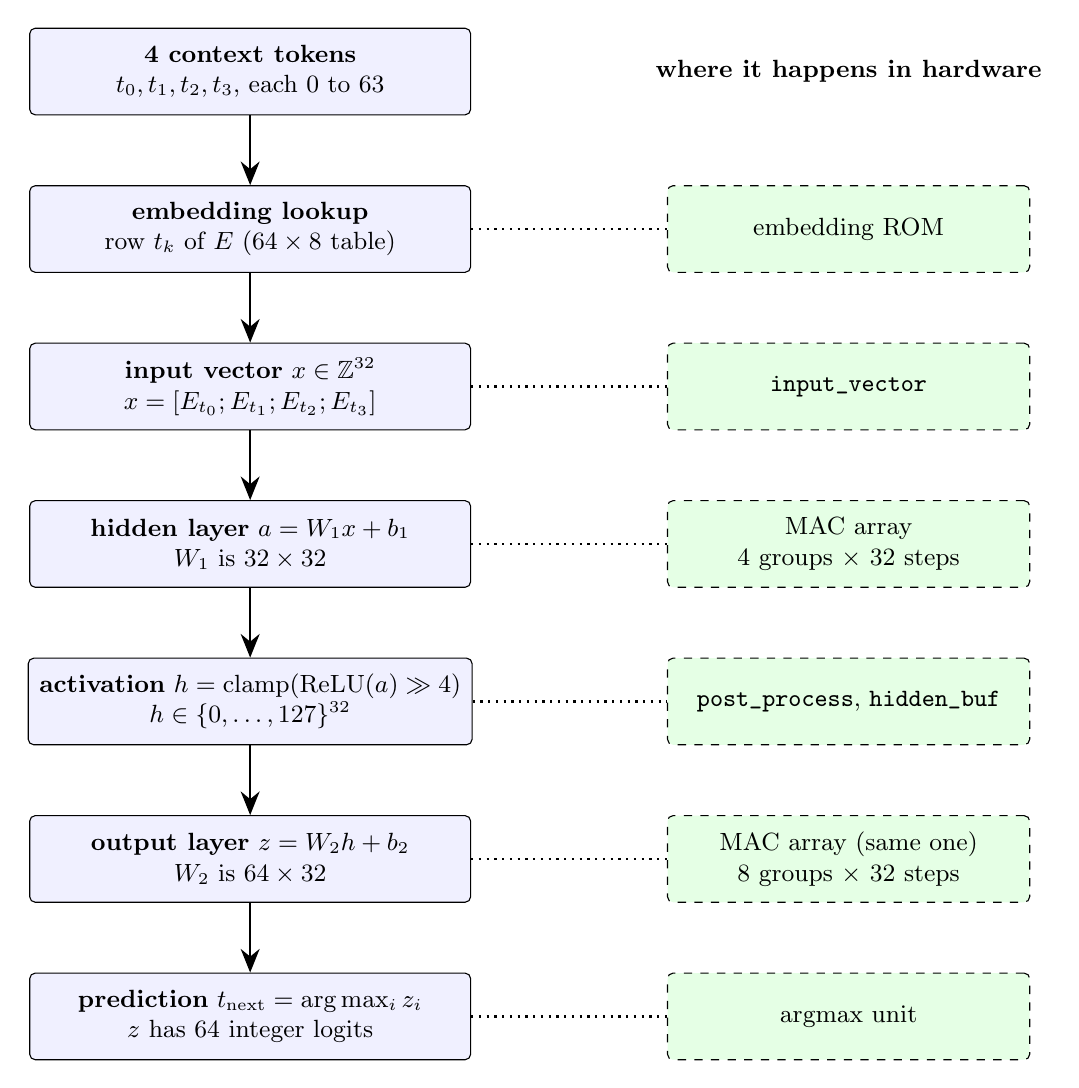
\begin{tikzpicture}
\node[box] (n0) at (0,0)     {\textbf{4 context tokens}\\$t_0,t_1,t_2,t_3$, each 0 to 63};
\node[box] (n1) at (0,-2.0)  {\textbf{embedding lookup}\\row $t_k$ of $E$ ($64\times 8$ table)};
\node[box] (n2) at (0,-4.0)  {\textbf{input vector} $x\in\mathbb{Z}^{32}$\\$x=[E_{t_0};E_{t_1};E_{t_2};E_{t_3}]$};
\node[box] (n3) at (0,-6.0)  {\textbf{hidden layer} $a=W_1x+b_1$\\$W_1$ is $32\times 32$};
\node[box] (n4) at (0,-8.0)  {\textbf{activation} $h=\mathrm{clamp}(\mathrm{ReLU}(a)\gg 4)$\\$h\in\{0,\dots,127\}^{32}$};
\node[box] (n5) at (0,-10.0) {\textbf{output layer} $z=W_2h+b_2$\\$W_2$ is $64\times 32$};
\node[box] (n6) at (0,-12.0) {\textbf{prediction} $t_{\mathrm{next}}=\arg\max_i z_i$\\$z$ has 64 integer logits};
\foreach \a/\b in {0/1,1/2,2/3,3/4,4/5,5/6}{\draw[data] (n\a) -- (n\b);}

\node[hw] (h1) at (7.6,-2.0)  {embedding ROM};
\node[hw] (h2) at (7.6,-4.0)  {\texttt{input_vector}};
\node[hw] (h3) at (7.6,-6.0)  {MAC array\\4 groups $\times$ 32 steps};
\node[hw] (h4) at (7.6,-8.0)  {\texttt{post_process}, \texttt{hidden_buf}};
\node[hw] (h5) at (7.6,-10.0) {MAC array (same one)\\8 groups $\times$ 32 steps};
\node[hw] (h6) at (7.6,-12.0) {argmax unit};
\foreach \k in {1,2,3,4,5,6}{\draw[dotted,thick] (n\k.east) -- (h\k.west);}
\node[font=\small\bfseries] at (7.6,0) {where it happens in hardware};
\end{tikzpicture}
\end{center}

The parameter count is $64\cdot 8 + (32\cdot 32+32) + (64\cdot 32+64) = 512+1056+2112 = 3680$. One forward pass costs $32\cdot 32 + 64\cdot 32 = 3072$ multiply-accumulates. With 8 lanes working side by side that is $3072/8 = 384$ accumulate steps, namely $4\cdot 32$ for the hidden layer and $8\cdot 32$ for the output layer.

\section*{2. Integer arithmetic: what each number means}

All stored values are integers that represent real numbers multiplied by a fixed scale.

\begin{center}
\begin{tabular}{@{}lllp{6.2cm}@{}}
\toprule
\textbf{Quantity} & \textbf{Type} & \textbf{Scale} & \textbf{Meaning} \\
\midrule
$E$, $W_1$, $W_2$, $x$, $h$ & INT8 & 16 & real value $=$ integer $/\,16$, so INT8 covers about $-8$ to $7.94$ \\
$b_1$, $b_2$ & INT32 & 256 & real value $=$ integer $/\,256$ \\
product $x_j\cdot W_{ij}$ & INT16 & 256 & scale $16\times 16$ \\
accumulator $a_i$, $z_i$ & INT32 & 256 & sum of products plus bias, all at scale 256 \\
\bottomrule
\end{tabular}
\end{center}

Why the numbers line up: a product of two scale-16 values has scale $16\cdot 16=256$, which is exactly the scale of the bias, so the bias can be added straight into the accumulator with no shifting.
The hidden layer produces $a$ at scale 256, but the output layer expects its input $h$ at scale 16 like every other INT8 value. Shifting right by 4 divides by 16, which converts scale 256 back to scale 16. The clamp to $[0,127]$ then keeps the result inside INT8, and the ReLU is the clamp's lower bound of 0.

The output layer does not need a shift. $W_2$ (scale 16) times $h$ (scale 16) plus $b_2$ (scale 256) gives logits at scale 256. The argmax does not care about the scale, since multiplying every logit by the same positive number never changes which one is largest.

\paragraph{Why 32 bits is enough.} Each accumulation sums 32 products, and each product has magnitude at most $128\cdot 128=2^{14}$. The sum is at most $32\cdot 2^{14}=2^{19}$ in magnitude, plus the bias. That is far below the INT32 limit of $2^{31}$, so the accumulator cannot overflow for any weights that fit in INT8.

\section*{3. A matrix-vector product, computed eight rows at a time}

The hidden layer asks for 32 outputs, each a dot product:
\[
a_i = b_i + \sum_{j=0}^{31} W_{ij}\,x_j .
\]
The hardware computes eight of these dot products at once. Output rows are grouped as $g=0,1,2,3$, where group $g$ holds rows $8g,\dots,8g+7$. For one group it runs $j$ from 0 to 31, and at each step it does
\[
a_{8g+k} \leftarrow a_{8g+k} + W_{8g+k,\,j}\;x_j \qquad k=0,\dots,7 .
\]
The single input $x_j$ is the same for all eight updates. Only the weight differs, and the eight weights are the slice of column $j$ belonging to group $g$.

\begin{center}
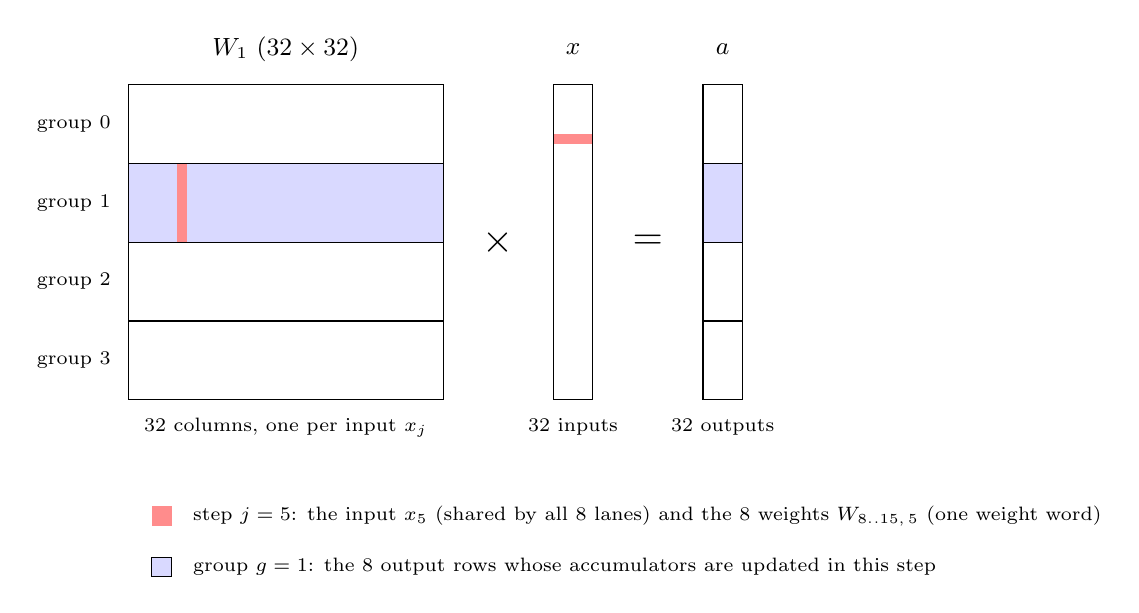
\begin{tikzpicture}[x=1cm,y=1cm]
% matrix W
\draw[fill=white] (0,0) rectangle (4,-4);
\foreach \r in {1,2,3}{\draw (0,-\r) -- (4,-\r);}
\fill[blue!15] (0,-1) rectangle (4,-2);
\fill[red!45] (0.625,-1) rectangle (0.75,-2);
\draw (0,0) rectangle (4,-4);
\foreach \r/\t in {0/{group 0},1/{group 1},2/{group 2},3/{group 3}}{
  \node[font=\scriptsize,anchor=east] at (-0.1,-\r-0.5) {\t};
}
\node[font=\small] at (2,0.45) {$W_1$ ($32\times 32$)};
\node[font=\scriptsize] at (2,-4.35) {32 columns, one per input $x_j$};
% x vector
\node[font=\Large] at (4.7,-2) {$\times$};
\draw[fill=white] (5.4,0) rectangle (5.9,-4);
\fill[red!45] (5.4,-0.625) rectangle (5.9,-0.75);
\draw (5.4,0) rectangle (5.9,-4);
\node[font=\small] at (5.65,0.45) {$x$};
\node[font=\scriptsize] at (5.65,-4.35) {32 inputs};
% equals
\node[font=\Large] at (6.6,-2) {$=$};
\draw[fill=white] (7.3,0) rectangle (7.8,-4);
\fill[blue!15] (7.3,-1) rectangle (7.8,-2);
\foreach \r in {1,2,3}{\draw (7.3,-\r) -- (7.8,-\r);}
\draw (7.3,0) rectangle (7.8,-4);
\node[font=\small] at (7.55,0.45) {$a$};
\node[font=\scriptsize] at (7.55,-4.35) {32 outputs};
% callouts
\fill[red!45] (0.3,-5.35) rectangle (0.55,-5.6);
\node[font=\scriptsize,anchor=west] at (0.7,-5.475) {step $j=5$: the input $x_5$ (shared by all 8 lanes) and the 8 weights $W_{8..15,\,5}$ (one weight word)};
\fill[blue!15] (0.3,-6.0) rectangle (0.55,-6.25);
\draw (0.3,-6.0) rectangle (0.55,-6.25);
\node[font=\scriptsize,anchor=west] at (0.7,-6.125) {group $g=1$: the 8 output rows whose accumulators are updated in this step};
\end{tikzpicture}
\end{center}

One \texttt{ACCUMULATE} cycle is exactly one column step: a single $x_j$ is multiplied by eight different weights and added into eight running sums. Walking $j$ from 0 to 31 completes the eight dot products of that group, and moving to the next group moves the blue band down by 8 rows.

The output layer uses the same machine with $h$ in place of $x$ and $W_2$ in place of $W_1$. The only differences are that it has eight groups instead of four ($W_2$ has 64 rows), and that its result goes to the argmax instead of being activated and stored.

\section*{4. The same computation as plain loops}

This is the integer reference the hardware must match bit for bit. The inner two loops are what the MAC array does in parallel.

\begin{verbatim}
x = concat(E[t0], E[t1], E[t2], E[t3])          # 32 INT8 values

for g in 0..3:                                   # hidden layer
    for k in 0..7:  acc[k] = b1[8*g + k]         # BIAS_LOAD
    for j in 0..31:                              # 32 ACCUMULATE steps
        for k in 0..7:                           # the 8 lanes, in parallel
            acc[k] += x[j] * W1[8*g + k][j]
    for k in 0..7:                               # post_process
        h[8*g + k] = min(max(acc[k], 0) >> 4, 127)

best_value = -2**31;  best_index = 0
for g in 0..7:                                   # output layer
    for k in 0..7:  acc[k] = b2[8*g + k]
    for j in 0..31:
        for k in 0..7:
            acc[k] += h[j] * W2[8*g + k][j]
    for k in 0..7:                               # argmax, in index order
        if acc[k] > best_value:                  # strict: ties keep the lower index
            best_value = acc[k];  best_index = 8*g + k
\end{verbatim}

\section*{5. A small worked example}

Take one lane with four inputs (a shortened version of the 32-step loop) and bias 100:
$x=[10,\,-3,\,7,\,2]$, $w=[5,\,4,\,-2,\,9]$.

\begin{center}
\begin{tabular}{@{}cccccc@{}}
\toprule
\textbf{step} & $x_j$ & $w_j$ & product & accumulator after \\
\midrule
bias load & & & & 100 \\
$j=0$ & 10 & 5 & 50 & 150 \\
$j=1$ & $-3$ & 4 & $-12$ & 138 \\
$j=2$ & 7 & $-2$ & $-14$ & 124 \\
$j=3$ & 2 & 9 & 18 & 142 \\
\bottomrule
\end{tabular}
\end{center}

The accumulator is 142, which at scale 256 is the real number $142/256\approx 0.555$. ReLU leaves it at 142 because it is positive. Shifting right by 4 gives $\lfloor 142/16\rfloor = 8$, and 8 is already inside $[0,127]$, so $h=8$, which at scale 16 is the real number $0.5$.

Two other outcomes of the same post-processing:
\begin{center}
\begin{tabular}{@{}lll@{}}
\toprule
\textbf{accumulator} & \textbf{after ReLU, shift 4} & \textbf{after clamp} \\
\midrule
$-258$ & ReLU gives 0, shift gives 0 & 0 \\
$3000$ & $3000\gg 4=187$ & 127 (clamped) \\
\bottomrule
\end{tabular}
\end{center}

The hardware realizes this without a comparator on the shifted value. For a non-negative accumulator, $a\gg 4>127$ exactly when $a\ge 2048$, which is exactly when some bit among $a[30:11]$ is set. Otherwise the answer is the seven bits $a[10:4]$. So the whole ReLU, shift, and clamp is a sign-bit test, one OR gate over 20 bits, and a bit selection.

\section*{6. One inference in math order, with cycle counts}

\begin{center}
\begin{tabular}{@{}p{4.1cm}p{8.4cm}r@{}}
\toprule
\textbf{FSM states} & \textbf{Math performed} & \textbf{Cycles} \\
\midrule
\texttt{EMBED_READ}, \texttt{EMBED_STORE} ($\times 4$) & $x[8k..8k+7]\leftarrow E_{t_k}$ for $k=0..3$ & 8 \\
\texttt{BIAS_READ}, \texttt{BIAS_LOAD} & $a_{8g+k}\leftarrow b1_{8g+k}$ for the 8 lanes & 2 \\
\texttt{WEIGHT_READ}, \texttt{ACCUMULATE} ($\times 32$) & $a_{8g+k}\mathrel{+}=W1_{8g+k,j}\,x_j$ for $j=0..31$ & 64 \\
\texttt{HIDDEN_STORE} & $h_{8g+k}\leftarrow\mathrm{clamp}(\mathrm{ReLU}(a_{8g+k})\gg 4)$ & 1 \\
\multicolumn{2}{@{}l}{\emph{those three rows repeat for groups $g=0..3$: $4\times 67=268$ cycles}} & \\
\texttt{BIAS_READ}, \texttt{BIAS_LOAD} & $z_{8g+k}\leftarrow b2_{8g+k}$ & 2 \\
\texttt{WEIGHT_READ}, \texttt{ACCUMULATE} ($\times 32$) & $z_{8g+k}\mathrel{+}=W2_{8g+k,j}\,h_j$ & 64 \\
\texttt{ARGMAX} ($\times 8$) & compare $z_{8g+k}$ with the best so far, one value per cycle & 8 \\
\multicolumn{2}{@{}l}{\emph{those three rows repeat for groups $g=0..7$: $8\times 74=592$ cycles}} & \\
\texttt{DONE} & report $t_{\mathrm{next}}=\text{best\_index}$ & 1 \\
\bottomrule
\end{tabular}
\end{center}

Total: $8+268+592+1=869$ cycles, about 8.7\,\textmu s at 100\,MHz.

\section*{7. What the Python side must agree on}

These are the places where a mismatch between the training script and the FPGA would silently give wrong tokens.
\begin{itemize}
\item \textbf{Scales and rounding:} $E$, $W_1$, $W_2$ quantized as $\mathrm{round}(16\cdot\text{real})$ and clamped to $[-128,127]$; biases as $\mathrm{round}(256\cdot\text{real})$ stored as INT32.
\item \textbf{Shift:} the post-activation shift is a floor division by 16 of a non-negative number, which is what an arithmetic right shift by 4 does.
\item \textbf{Concatenation order:} $x$ is $E_{t_0}$ first, then $E_{t_1}$, $E_{t_2}$, $E_{t_3}$, with element 0 of each embedding first.
\item \textbf{Weight layout:} the weight ROM word for (group $g$, input $j$) holds $W_{8g+k,\,j}$ for $k=0..7$ in bits $[8k+7:8k]$. In Python this is the transpose-and-pack of $W$ taken 8 rows at a time. Hidden-layer words come first (addresses 0 to 127), then output-layer words (128 to 383).
\item \textbf{Bias layout:} the bias ROM word for group $g$ holds $b_{8g+k}$ in bits $[32k+31:32k]$, hidden-layer words first (0 to 3), then output-layer words (4 to 11).
\item \textbf{Ties:} the argmax returns the lowest index among equal maxima, matching \texttt{numpy.argmax}.
\end{itemize}

\end{document}
